        
\documentclass[runningheads,a4paper]{llncs}
\def\spanishoptions{mexico}
\usepackage[spanish]{babel}

\usepackage{amssymb}
\setcounter{tocdepth}{3}
\usepackage{graphicx}
\usepackage[utf8]{inputenc}
\usepackage{url}
\usepackage{listings}
\usepackage[acronyms]{glossaries}
\setacronymstyle{long-short}

\makenoidxglossaries

%Terminos de glosario
\newglossaryentry{hacktivismo}{name={hacktivismo},
description={Es un acrónimo de hacker y activismo, se entiende normalmente "la utilización no-violenta de herramientas digitales ilegales o legalmente ambiguas persiguiendo fines políticos. Estas herramientas incluyen desfiguraciones de webs, redirecciones, ataques de denegación de servicio, robo de información, parodias de sitios web, sustituciones virtuales, sabotajes virtuales y desarrollo de software".}}

\newacronym{NSA}{NSA}{National Security Agency}
\newacronym{EE.UU}{EE.UU}{Estados Unidos de América}
\newacronym{CIU}{CIU}{The Competitive Intelligence Unit}
\newacronym{OEA}{OEA}{Organización de los Estados Americanos}
\newacronym{PF}{PF}{Policía Federal}
\newacronym{CMS}{CMS}{Content Management System}
\newacronym{LMS}{LMS}{Learning Management System}
\newacronym{LCMS}{LCMS}{Learning Content Management System}
\newacronym{TIC}{TIC}{Tecnologías de Información y Comunicaciones}
\newacronym{EDN}{EDN}{Estrategia Digital Nacional}
\newacronym{RTCE}{RTCE}{Reforma en Materia de Telecomunicaciones y Competencia Económica}
\newacronym{LTAIP}{LTAIP}{Ley de Transparencia y Acceso a la Información Pública}
\newacronym{LPD}{LPD}{Ley de Protección de Datos}
\newacronym{GRM}{GRM}{Gobierno de la República Mexicana}
\newacronym{PND}{PND}{Plan Nacional de Desarrollo}
\newacronym{SEN}{SEN}{Sistema Nacional de Educación}
\newacronym{LFTR}{LFTR}{Ley Federal de Telecomunicaciones y Radiodifusión}
\newacronym{LSPRM}{LSPRM}{Ley del Sistema Público de Radiodifusión de México}
\newacronym{TDT}{TDT}{Televisión Digital Terrestre}
\newacronym{IFT}{IFT}{Instituto Federal de Telecomunicaciones}
\newacronym{DOF}{DOF}{Diario Oficial de la Federación}
\newacronym{EUM}{EUM}{Estados Unidos Mexicanos}
\newacronym{LFPDPPP}{LFPDPPP}{Ley Federal de Protección de Datos Personales en Posesión de los Particulares}
\newacronym{IMC}{IMC}{Índice Mundial de Ciberseguridad}
\newacronym{ITU}{ITU}{International Telecomunication Union}
\newacronym{CMSI}{CMSI}{Cumbre Mundial sobre la Sociedad de la Información}
\newacronym{GCA}{GCA}{Global Cibersecurity Agenda}
\newacronym{MCA}{MCA}{Análisis Multicriterios}



\newcommand{\keywords}[1]{\par\addvspace\baselineskip
\noindent\keywordname\enspace\ignorespaces#1}

\begin{document}

\mainmatter  
\title{Antecedentes}
\titlerunning{Antecedentes}
\author{Ing. Felipe de Jesús Miramontes Romero}
\institute{Centro de Investigación en Matemáticas A.C.,\\Maestría en Ingeniería de Software,\\
Avenida Universidad 222, La Loma, 98068, Zacatecas, México.\\felipemiramontesr@gmail.com\\
\url{http://www.ingsoft.mx}}
\maketitle

\begin{abstract}
\keywords{Seguridad cibernetica, Delincuencia informática, México, Técnicas, Estrategias, Planes, Herramientas, Mejora de la Seguridad informática}
\end{abstract}

En esta sección es posible encontrar la información referente a los estudios y experimentos realizados para dar respuesta a la interrogante; ¿Cuál es el panorama general de la ciberseguridad en México? Para dar respuesta a la anterior cuestión y con el fin de realizar una propuesta en pro de la seguridad informática en el país se ha considerado identificar la información relacionada con las áreas de estudio utilizadas por la \gls{ITU} y ABI Research para la construcción \gls{IMC} \cite{GCSI_1}, cabe mencionar que la información de cada área de estudio sera enriquecida por medio de datos emanados de actividades y experimentos personales desarrollados con el objetivo de proveer un mayor nivel de detalle en el estudio. Ademas de lo mencionado anteriormente también es posible encontrar el planteamiento del problema, los objetivos generales y específicos así como la justificación de la presente propuesta.

\section{Marco teórico}

\subsection{Indice Mundial de Ciberseguridad (IMC)}
ABI Research \cite{GCSI_1} menciona que las \gls{TIC} son el catalizador que impulsa la evolución de las sociedades modernas pues sustentan el crecimiento social, económico y político de las personas, organizaciones y gobiernos. De igual manera se menciona que la tecnología y la Internet están ingresando de manera sistemática tanto en el ámbito publico como en el privado ya que estas proveen ventajas considerables en productividad, velocidad, reducción de costes y flexibilidad. Se menciona también que la ciberseguridad es de máxima importancia para el sostenimiento de cualquier modelo tecnológicamente aceptable pues los cibercriminales son numerosos, están bien organizados y ademas cuentan con medios de persuasión políticos, terroristas, hacktivistas (ver \gls{hacktivismo}), etc. Para lograr el progreso tecnológico, la ciberseguridad debe formar parte integral de cualquier proceso relacionado con la tecnología, sin embargo sigue sin formar parte fundamental de las estrategias tecnológicas nacionales e industriales, aunque en la actualidad es posible apreciar de manera táctil el avance tecnológico los esfuerzos en materia de seguridad informática siguen siendo eclécticos y dispersos. Se menciona que la solución se encuentra en la inserción de mecanismos de ciberseguridad en todos los estratos sociales, sin embargo a nivel global la diferencias económicas, políticas y de concientización entre Estados nación son una limitante, para remediar dicha situación es necesario realizar una comparativa entre las capacidades de la seguridad de cada país y la publicación de una clasificación efectiva de la situación pues de tal manera es posible revelar la deficiencias existentes y tomar un acicate para que se intensifiquen los esfuerzos en la materia. ABI Research \cite{GCSI_1} manifiesta que solo se puede sopesar el valor real de la capacidad de ciberseguridad de un país, por comparación y que el \gls{IMC} tiene como principal objetivo medir de manera efectiva el nivel de compromiso con la ciberseguridad de cada Estado nación, este se fundamenta en el mandato actual de la \gls{ITU} pues esta es un facilitador de la linea de acción C5 \cite{WSIS_1} de la \gls{CMSI} la cual tiene como propósito crear confianza y seguridad en la utilización de las \gls{TIC} a nivel nacional, regional e internacional. Se menciona también que el Dr. Hamadoun I. Touré Secretario General de \gls{ITU} en 2007, presento la \gls{GCA} como marco de cooperación entre las todas las partes interesadas en la construcción de una sociedad de la información mas segura. De acuerdo a Stein Schjolberg \cite{GCA_1} la \gls{GCA} es un marco de referencia para la cooperación internacional dirigida a la mejora de la confianza y seguridad en una sociedad de la información, se basa en 5 áreas de trabajo: medidas jurídicas, medidas técnicas, medidas de organización, creación de capacidades y cooperación.\\

El modelo estadístico utilizado para la asignación del \gls{IMC} se inspira en el \gls{MCA} así lo menciona ABI Research \cite{GCSI_1}, el \gls{MCA} establece la preferencia entre alternativas por referencia a un grupo explícito de objetivos para los que se han definido criterios de evaluación del grado en el que sean alcanzados dichos objetivos, se aplica un modelo de evaluación lineal aditiva, la matriz de rendimiento describe las alternativas y las columnas el rendimiento de las alternativas en relación a los criterios. La puntuación de la evaluación comparativa se apoya en indicadores ponderados de manera equitativa, se otorgan 0 puntos cuando no existen actividades; 1 cual la medida posee carácter parcial; y 2 puntos para medidas de alto alcance. La puntuación total de las categorías es la siguiente (Figura 1):  

\begin{figure}
\centering
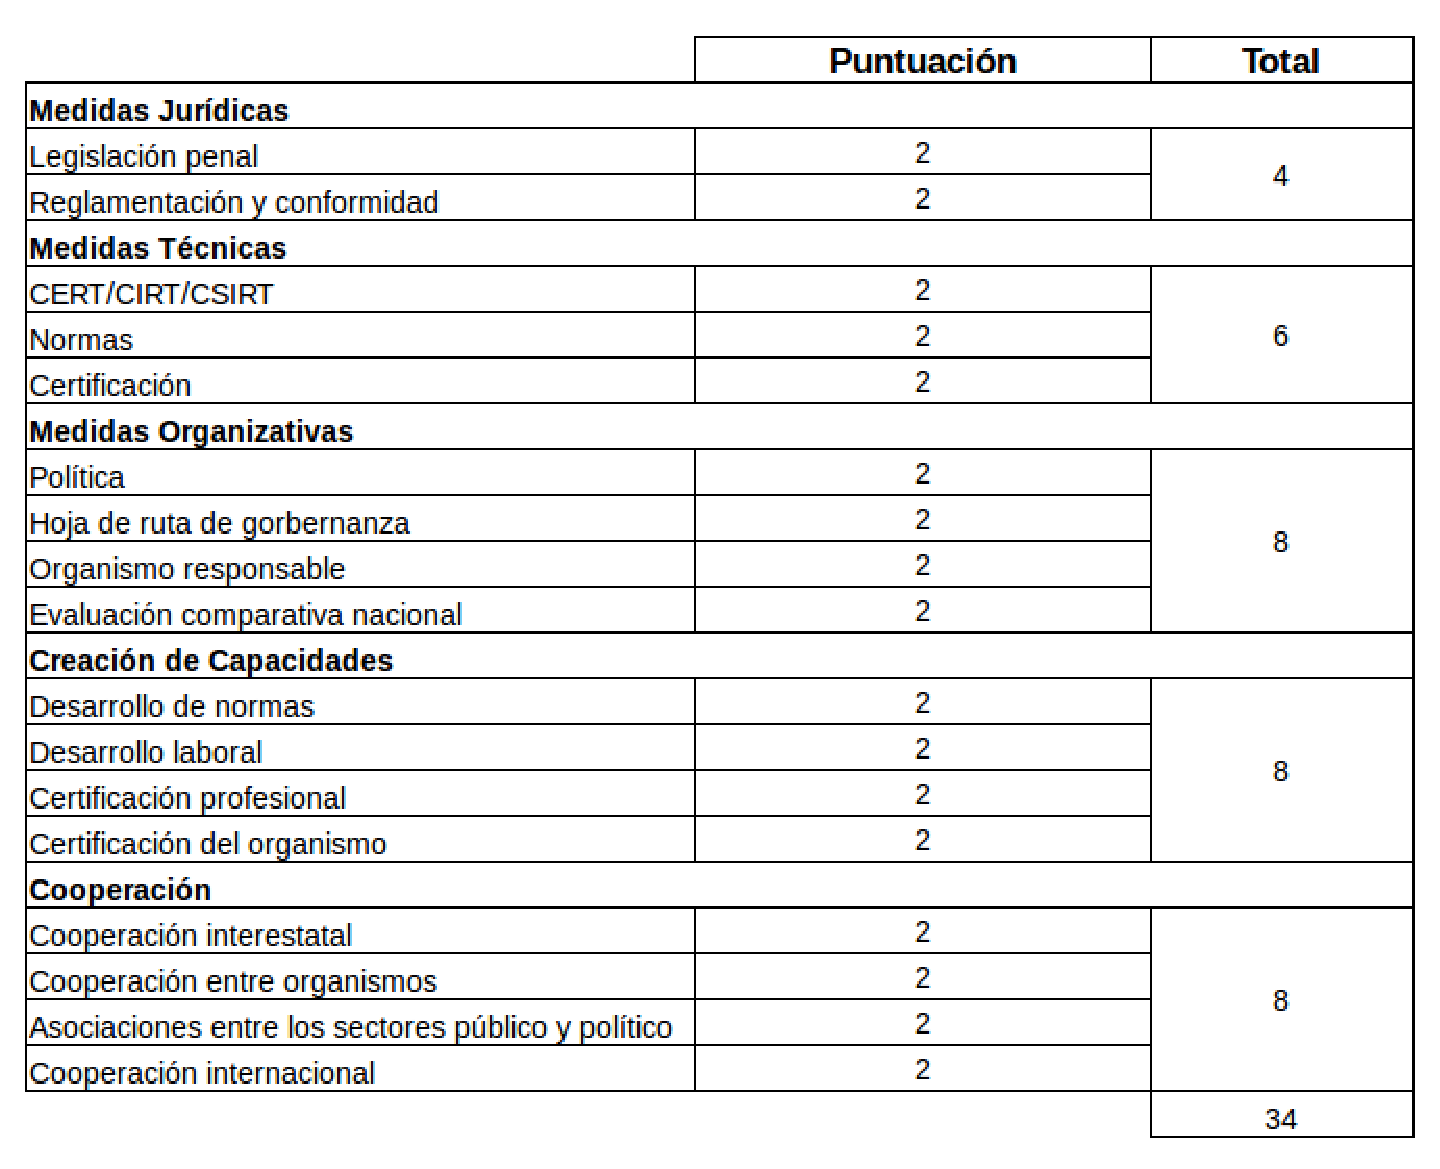
\includegraphics[height=12cm, width=12.0cm]{imc_indicadores}
\caption{Puntuación total atribuida a cada una de las categorías del Indice Mundial de Ciberseguridad (IMC).}
\label{fig:example}
\end{figure}



\subsection{Medidas Jurídicas- Visión Tecnológica de un País en Desarrollo}
En el texto denominado Estrategia Digital Nacional \cite{EDN_1} se dice que el gobierno mexicano ha establecido como propósito fundamental magnificar el impacto positivo ejercido por las \gls{TIC} en el área social, económica y política del país. Esto con el fin de mejorar la calidad de vida y el bienestar social de los ciudadanos mexicanos. Para ello se han realizado esfuerzos puntuales que pretenden establecer un universo normativo que promueva la utilización de nuevas tecnologías de manera segura. Dentro de dichos esfuerzos es posible identificar como ejes principales a las nuevas leyes, reformas y estrategias impulsadas por el gobierno en los últimos años, entre las cuales se destaca la \gls{EDN}, la \gls{RTCE}, la \gls{LTAIP} y la \gls{LPD}.  

\subsubsection{Estrategia Digital Nacional (EDN)}  
En \cite{EDN_1} se dice que la \gls{EDN} es un documento descriptivo que contiene los detalles referentes a las acciones que el \gls{GRM} implementará durante los próximos años para fomentar la adopción y el desarrollo de las TIC e insertar a México en la Sociedad de la Información y el Conocimiento, ademas fungirá como una guía de acciones a través de la cual se medirán los avances, logros y retos referentes a la temática.\\ 

La intención de la \gls{EDN} es aumentar la digitalización de México, para que
con ello se maximice su impacto económico, social y político en beneficio de la calidad de vida de
las personas. En \cite{EDN_1} se dice que es necesario que las tecnologías sean aprovechadas para mejorar diversos aspectos de la vida de las personas. Ademas se dice que ``en la medida en que los individuos, empresas y gobierno integren y adopten las TIC en sus actividades cotidianas, habrá mejoras en la calidad de vida de las personas, en la eficiencia de los procesos productivos de las empresas y en la eficiencia de los procesos de gestión, provisión de servicios públicos, transparencia y rendición de cuentas del gobierno''.\\

\cite{EDN_1} menciona que a partir del objetivo, la misión y la visión de la Estrategia Digital Nacional (EDN) son las siguientes:

\begin{itemize}
	\item Misión: Facilitar el acceso y promover la utilización de las TIC en la vida cotidiana de la
sociedad y del gobierno para que éstas contribuyan al desarrollo económico y social del
país, y a mejorar la calidad de vida de las personas.\\
	\item Visión: Un México Digital con una sociedad conectada, participativa e innovadora que
potencializa sus capacidades para tener mejores oportunidades; y un gobierno abierto,
cercano, moderno y transparente, que garantice que la tecnología sea motor del desarrollo del país.
\end{itemize}

En \cite{EDN_1} se dice que a partir de su objetivo principal la estrategia 5 objetivos ligados a las metas nacionales planteadas en el \gls{PND} 2013 - 2018 y a continuación son descritos de manera general.\\

\begin{enumerate}
	\item Transformación gubernamental: ``Construir una nueva relación entre la sociedad y el gobierno,
centrada en la experiencia del ciudadano como usuario de servicios públicos, mediante la adopción del uso de las TIC en el Gobierno de la República. Desarrollar un ecosistema de economía digital que contribuya a alcanzar un México próspero, mediante la asimilación de las \gls{TIC} en los procesos económicos, para estimular el aumento de la productividad, el crecimiento económico y la creación de empleos formales''.\\
	\item Economía digital: ``Desarrollar un ecosistema de economía digital que contribuya a alcanzar un México próspero, mediante la asimilación de las \gls{TIC} en los procesos económicos, para estimular el aumento de la productividad, el crecimiento económico y la creación de empleos formales''.\\
	\item Educación de calidad: ``Integrar las \gls{TIC} al proceso educativo, tanto en la gestión educativa como en los procesos de enseñanza-aprendizaje, así como en los de formación de los docentes y de difusión y preservación de la cultura y el arte, para permitir a la población insertarse con éxito en la Sociedad de la Información y el Conocimiento''.\\
	\item Salud universal y efectiva: ``Generar una política digital integral de salud que aproveche las oportunidades que brindan las \gls{TIC} con dos prioridades: por una parte, aumentar la cobertura, el acceso efectivo y la calidad de los servicios de salud y, por otra, hacer más eficiente el uso de la infraestructura instalada y recursos destinados a la salud en el país''.\\
	\item Seguridad ciudadana: ``Utilizar a las \gls{TIC} para prevenir la violencia social, articulando los esfuerzos de la ciudadanía y de las autoridades en torno a objetivos comunes para promover la seguridad, y también para prevenir y mitigar los daños causados por desastres naturales''.
\end{enumerate}

Para asegurar el cumplimiento de los objetivos el Gobierno de la República propone en \cite{EDN_1} los siguientes habilitadores.

\begin{enumerate}
	\item Conectividad: ``Desarrollo de redes y la ampliación del despliegue de una mejor infraestructura en el territorio nacional, la ampliación de la capacidad de las redes existentes, y el desarrollo de competencia en el sector de \gls{TIC} para estimular la reducción de precios''.\\
	\item Inclusión y habilidades digitales: ``Se refiere al desarrollo equitativo de habilidades para operar
tecnologías y servicios digitales, contemplando la cobertura social y el desarrollo de habilidades con equidad de género''.\\
	\item Interoperabilidad: ``Se refiere a las capacidades técnicas, organizacionales, de gobernanza y semánticas, necesarias en los sistemas tecnológicos para compartir información y transacciones de forma
consistente''.\\
	\item Marco jurídico: ``Se refiere a la armonización del marco jurídico con la finalidad de propiciar un entorno de certeza y confianza favorables para la adopción y fomento de las \gls{TIC}''. En \cite{EDN_1} se dice que el habilitador tiene la finalidad de propiciar un entorno de certeza y confianza para la adopción y fomento de las \gls{TIC} lo que implica el análisis del marco jurídico en torno a los diversos temas que contempla la Estrategia, entre los cuales están:\\
	\begin{enumerate}
		\item Protección de los derechos humanos.
		\item Gobernanza de Internet.
		\item Privacidad y protección de datos personales.
		\item Seguridad de la información y delitos informáticos.
		\item Firma Electrónica Avanzada.
		\item Comercio electrónico.
		\item Propiedad intelectual.
		\item Gobierno digital.
		\item Educación y salud digitales.
		\item Economía digital.\\
	\end{enumerate}
	
	\item Datos abiertos: ``Se refiere a la disponibilidad de información gubernamental en formatos útiles y reutilizables por la población en general, para fomentar el emprendimiento cívico e impulsar la transparencia, mejorar los servicios públicos y detonar mayor rendición de cuentas''.
\end{enumerate}  

En \cite{EDN_1} se dice que para lograr el objetivo ``Transformación Gubernamental'' sera necesario impulsar acciones para mejorar la eficiencia gubernamental, la transparencia pública y la rendición de cuentas así como la capacidad de repuesta del gobierno, dichas actividades son listadas como objetivos secundarios  a continuación.

\begin{enumerate}
	\item Generar y coordinar acciones orientadas hacia el logro de un gobierno abierto.
	\item Instrumentar la ventanilla única nacional para tramites y servicios.
	\item Crear una política de \gls{TIC} sustentable para la administración pública federal.
	\item Instrumentar una política digital del territorio nacional.
	\item Usar datos para el desarrollo y el mejoramiento de políticas públicas.
	\item Adoptar una comunicación digital centrada en el ciudadano.
\end{enumerate}

En \cite{EDN_1} se dice que para lograr el objetivo ``Economía Digital'' sera necesario sera necesario articular políticas púbicas para promover la oferta y la demanda de bienes y servicios digitales ademas de la adopción de las \gls{TIC} en procesos digitales, dichos esfuerzos son listados como objetivos secundarios a continuación.

\begin{enumerate}
	\item Desarrollar el mercado de bienes y servicios digitales.
	\item Potenciar el desarrollo del comercio electrónico.
	\item Estimular la innovación de servicios digitales a través de la democratización del gasto público.
	\item Asegurar la inclusión financiera mediante esquemas de banca móvil.
\end{enumerate}

En \cite{EDN_1} se dice que para lograr el objetivo ``Educación de Calidad'' se deberá promover el uso de las \gls{TIC} las cuales incrementaran el rendimiento y la oferta educativa, se deberá realizar actividades encaminadas en proveer de habilidades digitales a profesores y alumnos, ademas se deberá promover la creación y difusión dela cultura digital, las actividades propuestas son listadas como objetivos secundarios a continuación.

\begin{enumerate}
	\item Desarrollar una política nacional de adopción y uso de las \gls{TIC} en el proceso de enseñanza-aprendizaje del \gls{SEN}.
	\item Ampliar la oferta educativa a través de medios digitales.
	\item Desarrollar una agenda digital de cultura.
	\item Mejorar la gestión educativa mediante el uso de las \gls{TIC}.
\end{enumerate}

En \cite{EDN_1} se dice que para lograr el objetivo ``Salud Universal y Efectiva'' sera necesario el uso de las \gls{TIC} para contribuir al acceso universal y afectivo a los servicios de salud, las actividades que deberán ser implementadas pueden ser listadas como objetivos secundarios a continuación.

\begin{enumerate}
	\item Incorporar el uso de las \gls{TIC} para facilitar la convergencia de los sistemas de salud y ampliar la cobertura en los servicios de salud.
	\item Establecer la personalidad única en salud a través del padrón general de salud.
	\item Implementar Sistemas de Información de Registro Electrónico para la Salud.
	\item Implementar el Expediente Clínico Electrónico (ECE), el Certificado Electrónico de Nacimiento (CeN) y la Cartilla Electrónica de Vacunación (CeV).
	\item Instrumentar mecanismos de Telesalud y Telemedicina.
\end{enumerate}

En \cite{EDN_1} se dice que para lograr el objetivo ``Seguridad Ciudadana'' sera necesario el fortalecimiento de los marcos institucionales y de política que permitan reforzar y consolidar la seguridad ciudadana, las actividades que deberán ser implementadas pueden ser listadas como objetivos secundarios a continuación.

\begin{enumerate}
	\item Generar herramientas y aplicaciones de denuncia ciudadana en múltiples plataformas.
	\item Desarrollar instrumentos digitales para la prevención social de la violencia.
	\item Impulsar la innovación cívica por medio de las \gls{TIC}.
	\item Prevenir y mitigar los daños causados por desastres naturales mediante el uso de las \gls{TIC}.
\end{enumerate}

Para ver mas detalles de la Estrategia Digital Nacional (EDN) es necesario acudir a la siguiente fuente digital: \url{http://goo.gl/VPaIUr}.

\subsubsection{Reforma en Materia de Telecomunicaciones y Competencia Económica (RTCE)}
En el documento denominado ``Explicación de la Reforma en Materia de Telecomunicaciones y Competencia Economica'' \cite{RMT_1} se menciona que el Presidente de la Republica Enrrique Peña Nieto envió a la camara de senadores la iniciativa de decreto por el que se expide la \gls{LFTR} y la \gls{LSPRM} el día 24 de marzo del 2014, dicha iniciativa derivó de la reforma constitucional a los artículos, 6o, 7o, 27, 28, 73, 78, 94 y 105 de la Constitución Política de los Estados unidos Mexicanos. Los diputados y senadores aprobaron la iniciativa el día 14 de julio del 2014 la cual fue modificada con el fin de enriquecer su contenido.\\

La reforma expedida en el mes de junio del 2013 se encuentra basada en 6 bases rectoras.

\begin{enumerate}
	\item Emisión de un nuevo marco legal.
	\item Reglas específicas para la competencia efectiva.
	\item Fortalecimiento de las instituciones involucradas en los sectores de telecomunicaciones y
radiodifusión.
	\item Objetivos específicos para la cobertura universal de los servicios.
	\item Despliegue de infraestructura.
	\item Ampliación de los derechos fundamentales de libertad de expresión, acceso a la informa-
ción y a las tecnologías de la información y comunicación.
\end{enumerate}

En \cite{RMT_1} se dice que uno de los propósitos fundamentales de la legislación secundaria es; fusionar y actualizar en una sola ley la Ley Federal de Radio y Televisión, que data de 1960, y la Ley Federal de Telecomunicaciones, expedida en 1995, ademas de modificar otras 11 leyes con el fin de armonizarlas con los nuevos ordenamientos legales. Así mismo se dice que las nuevas normativas son entes orgánicos que utilizan como eje rector las necesidades del usuario de los servicios que la ley ampara. Ademas se puntualizan los beneficios concretos a los cuales los mexicanos podrán acceder, entre los cuales se encuentran los siguientes: \\

\begin{enumerate}
	\item ``Mas y mejores derechos''. \\
	\item ``Mas y mejores derechos para las audiencias''.\\
	\item ``Mas y mejores derechos para las audiencias con discapacidad''.\\
	\item ``Dos nuevas cadenas de televisión digital abierta, a efecto de incrementar la competencia 	
en el sector de la radiodifusión''.\\
	\item ``Desaparición de los cobros por el servicio telefónico de larga distancia''.\\
	\item ``La posibilidad de mantenerse comunicado cuando el usuario de telefonía móvil se
encuentre fuera del área de cobertura contratada, con independencia del operador que le preste los servicios''.\\
	\item ``La eliminación de la tarifa que aplicaba el operador móvil preponderante por el servicio de 	
“usuario visitante” o roaming, y la consecuente reducción o eliminación de dicha tarifa por parte de sus competidores''.\\
	\item ``Mayor competencia, que implica más servicios, con mejor calidad y a buenos precios''.\\
	\item ``Desaparición en 2015 de las señales tradicionales de televisión, para transitar a la 
\gls{TDT}, lo cual implica tener acceso a audio y video de mayor 	calidad, así como multiplicar el número de canales transmitidos, aumentando la disponibilidad de programación y contenidos, y liberando espectro para ser utilizado con otros fines''.\\
	\item ``Un nuevo organismo público descentralizado de radiodifusión, denominado Sistema de Radiodifusión del Estado Mexicano, que asegure la difusión de información imparcial, objetiva, oportuna y veraz, así como la expresión de la diversidad y pluralidad de ideas y opiniones''.\\
	\item ``Apertura a la inversión extranjera directa (hasta el 100 por ciento en telecomunicaciones y hasta el 49 por ciento en radiodifusión), para fortalecer la competencia, así como acceder a tecnologías avanzadas y a nuevos modelos de negocio y de comercialización de los servicios''.\\
	\item ``Conectividad en sitios públicos, tales como escuelas, centros de salud y oficinas de gobierno, así como condiciones para el desarrollo de una red nacional de educación e investigación interconectada nacional e internacionalmente''.\\
	\item ``Una nueva red troncal que ampliará la red de fibra óptica de la Comisión Federal de 	Electricidad y una nueva red compartida de servicios móviles en la banda de 700 MHz''.
\end{enumerate}

En \cite{RMT_1} se dice que el diseño institucional es una de las razones que motivaron al desarrollo de la iniciativa pues se identifico que en una misma materia concurrían de 2 a 4 autoridades con diferentes enfoques lo que generaba un problema denominado ``Doble Ventanilla''. Para dar solución a dicha problema fue creado el \gls{IFT} como órgano constitucional autónomo con personalidad jurídica y patrimonio propios, que tiene por objeto el desarrollo eficiente de la radiodifusión y las telecomunicaciones conforme a lo dispuesto en la Constitución, así como en los términos que fijan las leyes. El gobierno afirma en \cite{RMT_1} que el trafico promedio mensual móvil a nivel mundial sera 10 veces superior en el 2018; en latinoamerica el crecimiento sera 12 veces mayor, considerando lo anterior se ha estipulado que el espectro radioeléctrico deberá planificarse para que pueda ofrecer mas y mejores servicios, ademas la ley plantea un nuevo proceso para la obtención de concesiones sobre los recursos orbitales futuros. En cuanto al tema de las concesiones la reforma constitucional propone un proceso especial que da los parámetros para su otorgamiento. La reforma menciona que en México el sector de las telecomunicaciones se ha caracterizado por sus altos precios lo cual ha potencializando el bajo porcentaje de penetración de los servicios y un deficiente desarrollo de la infraestructura, en \cite{RMT_1} se menciona que un objetivo de la reforma es llegar a todas las regiones del país con redes de telecomunicaciones par promover el desarrollo económico y la inclusión social por medio de la activación del sector privado, para tal efecto la ley marca que los concesionarios de redes de telecomunicaciones para uso comercial deberán adoptar diseños de arquitectura abierta de red con el fin de promover la interconexion e interoperabilidad de sus redes, de manera puntual la ley dice que la información transmitida a través de las nuevas redes y servicios deberán cumplir con el principios de confidencialidad y privacidad.\\

Para ver mas detalles de la Reforma de Telecomunicaciones y Competencia Económica (RTCE) es necesario acudir a la siguiente fuente digital: \url{http://goo.gl/7uSn4L}.

\subsubsection{Ley de Transparencia y Acceso a la Información Pública Gubernamental (LTAIP)}
En el capítulo I, artículo 1 de \cite{LTAIP_1} se dice que la \gls{LTAIP} tiene como finalidad promover el acceso de toda persona a la información en posesión de los Poderes de la Unión, los órganos constitucionales autónomos y con autonomía legal ademas de cualquier otra entidad federal. En el artículo 5 se menciona que la ley es de observancia obligatoria para los servidores públicos federales, mientras los servidores públicos estatales se rigen bajo la propia ley de cada estado.\\

Por otra parte en cuanto a las obligaciones de transparencia, en el capítulo II, artículo 7 de \cite{LTAIP_1} se dice que los sujetos obligados deberán poner a disposición del público y actualizar, en términos del reglamento y los lineamientos que expida el instituto o instancia equivalente la siguiente información:

\begin{itemize}
	\item Estructura orgánica.
	\item Facultades de cada unidad administrativa.
	\item Directorio de servidores públicos, desde el nivel de jefe de departamento.
	\item Remuneración mensual por puesto, incluso el sistema de compensación.
	\item El domicilio de la unidad de enlace, dirección electrónica donde deberán recibirse las solicitudes para obtener información.
	\item Metas y objetivos.
	\item Los servicios que ofrecen.
	\item Tramites, requisitos y formatos.
	\item La información sobre el presupuesto asignado, así como los informes de su ejecución. 
	\item Los resultados de auditorias al ejercicio presupuestal de cada sujeto obligado.
	\item El diseño, ejecución, montos asignados y criterios de acceso a los programas de subsidio.
	\item Las concesiones, permisos o autorizaciones otorgados, especificando los titulares de aquéllos.
	\item Las contrataciones que se hayan celebrado en términos de la legislación aplicable detallando por
cada contrato:
		\begin{itemize}
			\item El monto,
			\item El nombre del proveedor, contratista o de la persona fisica o moral con quienes se haya celebrado el contrato y;
			\item Los plazos de cumplimiento de los contratos;
		\end{itemize}
	\item El marco normativo aplicable a cada sujeto obligado.
	\item Los informes generados.
	\item Los mecanismos de participación ciudadana.
	\item Cualquier información que sea de utilidad o se considere relevante.
\end{itemize}

En el artículo 9 de \cite{LTAIP_1} se dice que la información que se refiere en el artículo 7 deberá de encontrarse a disposición de los ciudadanos a través de medios remotos o locales de comunicación electrónica, ademas se puntualiza que; ``los sujetos obligados deberán tener a disposición de las personas interesadas equipo de cómputo, a fin de que éstas puedan obtener la información, de manera directa o mediante impresiones. Asimismo, éstos deberán proporcionar apoyo a los usuarios que lo requieran y proveer todo tipo de asistencia respecto de los trámites y servicios que presten''.\\

El artículo 12 de \cite{LTAIP_1} menciona que los sujetos obligados deberán publicar la información relativa a los montos y las personas a quienes se entregan, por cualquier motivo, recursos públicos, así como los informes del destino de dichos recursos.\\

En cuanto al tema de información reservada y confidencial en el artículo 13 de \cite{LTAIP_1} se menciona que la información reservada es aquella que pueda:

\begin{itemize}
	\item Comprometer la seguridad nacional, pública o la defensa nacional.
	\item Menoscabar la conducción de negociaciones internacionales.
	\item Dañar la estabilidad financiera del país.
	\item Poner el riesgo la vida, la seguridad o la salud de cualquier persona.
	\item Causar perjuicio a al cumplimiento de las leyes, prevención y persecución de delitos.	
\end{itemize}

Por otra parte en el artículo 14 también se considera como información reservada los siguientes puntos:
\begin{itemize}
	\item La que por disposición de una ley se considere confidencial, reservada o comercial.
	\item Los secretos comerciales, industriales, fiscales, bancartios, fiduciarios u otro considerado como tal por alguna ley.
	\item Las averiguaciones previas.
	\item Los expedientes judiciales.
	\item Los procedimientos de responsabilidad de los servidores públicos.
	\item La información que contenga opiniones, recomendaciones o puntos de vista que formen parte del proceso deliberativo de los servidores públicos.
\end{itemize}

En el artículo 15 de \cite{LTAIP_1} se dice que la información reservada podrá permanecer con tal caracter hasta por un periodo de 12 años. \\

Por otra parte en el artículo 18 de \cite{LTAIP_1} se menciona que la información confidencial es aquella que ha sido entregada con tal carácter por los particulares a sujetos obligados, de conformidad con el artículo 19, los datos personales que requieran consentimiento de los individuos para su difusión, distribución o comercialización.\\

La \gls{LTAIP} posee como característica particular una sección puntual acerca de la protección de datos personales, en el artículo 20 se dice que; los sujetos obligados serán responsables de los datos personales y deberán:

\begin{itemize}
	\item Adoptar procedimientos adecuados para recibir y responder las peticiones realizadas por parte de los ciudadanos, así como capacitar a los servidores públicos de dar a conocer información sobre las politicas de protección de datos.
	\item Tratar los datos personales solo cuando sea pertinente en realación con los propositos para los cuales se hayan obtenido.
	\item Poner a disposición inmediata los propósitos del tratamiento de los datos.
	\item Procurar cumplir con el principio de exactitud y actualización.
	\item Tratar los datos personales que fueren inexactos.
	\item Adoptar las medidas necesarias que garanticen la seguridad de los datos personales y eviten su
alteración, pérdida, transmisión y acceso no autorizado. 
\end{itemize}

Por otra parte el artículo 22 de \gls{LTAIP} estipula que no sera requerido ningún consentimiento de los individuos para proporcionar datos personales en los siguientes casos:

\begin{itemize}
	\item Por razones estadísticas, científicas de interés general previstas en la ley, previo procedimiento por el cual no sea posible asociar datos con individuos.
	\item Cuando se transmitan entre sujetos obligados siempre y cuando los datos sean utilizados para el ejercicio de facultades propias.
	\item Para cumplir con un orden judicial.
	\item A terceros cuando se contrate la prestación de un servicio que requiera el tratamiento de datos personales.
	\item En los demás casos que establezcan las leyes.
\end{itemize}

Para ejercer un control administrativo la \gls{LTAIP} en contiene una sección de responsabilidades y sanciones donde en su artículo 63 menciona que serán causas de responsabilidad administrativa de los servidores públicos por incumplimiento de las obligaciones establecidas en la ley las siguientes:

\begin{itemize}
	\item Usar, sustraer, destruir, ocultar, inutilizar, divulgar o alterar, total o parcialmente y de manera indebida información que se encuentre bajo su custodia y a la cual tengan acceso o conociemiento con motivo de su empleo, cargo o comisión.
	\item Actuar con negligencia, dolo o mala fe en la sustanciación de las solicitudes de acceso a la información o en la difusión de la información a que están obligados conforme a esta ley.
	\item Denegar intencionalmente la información pública.
	\item Clasificar como reservada información inadecuada.
	\item Entregar información clasificada con dolo y mala fe.
	\item Entregar intencionalmente de manera incompleta información requerida.
	\item No proporcionar la información requerida por órganos referidos en la fracción IV de la ley o el Poder de la Federación.
\end{itemize}

Las responsabilidades administrativas generadas por el incumplimiento son independientes del orden civil y penal así lo menciona el artículo 64 de la \gls{LTAIP}.

\subsubsection{Ley Federal de Protección de Datos Personales en Posesión de los Particulares (LFPDPPP)}
En el texto \cite{LFPDPPP_1} se dice que el 5 de julio del 2010 fue publicada en el \gls{DOF} la \gls{LFPDPPP}, siendo presidente de la república el C. Felipe de Jesús Calderón Hinojosa.\\

En el articulo 1 de \cite{LFPDPPP_1} se menciona que la ley es de orden púbico y de observancia general en todo el país y que tiene como objetivo la protección de los datos personales en posesión de los particulares, por medio del tratamiento legitimo, controlado e informado para garantizar la privacidad y el derecho de autodeterminación informativa de las personas. En el artículo 2 se dice que son sujetos obligados las personas físicas, morales y de carácter privado, con excepción de sociedades crediticias y las personas que lleven a cabo recolección de datos personales sin fines de divulgación.\\

En el capítulo II de \cite{LFPDPPP_1} es tratada la sección relacionada a los principios de protección de datos personales, en el artículo 6 se dice que los responsables del tratamiento de datos personales deberán cumplir con los principios de; licitud, consentimiento, información, calidad, finalidad, proporcionalidad y responsabilidad. En cuanto al tratamiento de los datos el artículo 7 menciona que para todo tratamiento de datos sera necesario cumplir con la expectativa de privacidad. Por otra parte el artículo 8 menciona los casos en los cuales el tratamiento de los datos no estará sujeto al consentimiento de titular y acontinuación son mencionados:

\begin{itemize}
	\item Previo consentimiento expreso, verbalmente, por escrito. por medios electrónicos, ópticos y cualquier otra tecnología, o por signos inequívocos.
	\item Por aceptación de aviso de privacidad.
	\item En los casos incluidos en los artículos 10 y 37 de la presente Ley.
\end{itemize}

Tratándose de datos personales del tipo sensibles se deberá obtener el permiso del titular por medio de firma autógrafa, firma electrónica, o cualquier mecanismo de autenticación así lo manifiesta el articulo 9, ademas de ello manifiesta que no podrán crear bases de datos sensibles sin tener el correcto justificativo. Por otra parte el artículo 10 dice que no sera necesario el consentimiento para el tratamiento de los datos personales en los siguientes casos:

\begin{itemize}
	\item Cuando este previsto por la Ley.
	\item Cuando la información se encuentre incluida dentro de las fuentes de acceso público.
	\item Cuando los datos estén sometidos disociación.
	\item Por obligaciones derivadas de una relación jurídica entre el titular y el responsable.
	\item Alguna situación de emergencia que ponga en riesgo a un individuo en persona y bienes.
	\item Cuando la información sea necesaria para la atención medica.
	\item Cuando lo dicte la autoridad competente.
\end{itemize}    
  
En el artículo 11 se dice que el responsable de las bases de datos deberá cumplir con la pertinencia, correctitud y la actualización de la información, se dice también que cuando los datos han dejado de ser necesarios deben ser cancelados, por otra parte el artículo 12 menciona que el tratamiento de los datos debe limitarse a lo señalado en el aviso de privacidad y si el tratamiento de los datos es inevitable deberá obtenerse la autorización del titular con anterioridad. Por su parte el artículo 13 menciona que los datos deberán ser sometidos al tratamiento necesario, adecuado y relevante en relación con las finalidades previstas en el aviso de privacidad.\\    

El responsable de la protección de datos personales deberá velar por el cumplimiento de los principios establecidos por la ley por medio de la adopción de las medidas necesarias, ademas de ello sera necesario garantizar que el aviso de privacidad sea respetado en todo momento así lo estipula el artículo 14 de \cite{LFPDPPP_1}, por su parte el artículo 15 menciona que sera necesario informar a los titulares la información que se recaba de ellos por medio de aviso de privacidad el cual contener los siguientes datos según el artículo 16: 

\begin{itemize}
	\item La identidad y domicilio del responsable.
	\item La finalidades del tratamiento.
	\item Las opciones que el responsable ofrezca a los titulares para limitar el uso y divulgación.
	\item Los medio para ejercer derechos de acceso, rectificación, cancelación u oposición.
	\item Las transferencias de datos que se efectúen.
	\item El procedimiento y medio por el cual se dará aviso sobre cambios en aviso de privacidad.
\end{itemize}

En cuanto a al artículo 19 de \cite{LFPDPPP_1} se menciona que, ``todo responsable que lleve a cabo tratamiento de datos personales deberá establecer y mantener medidas de seguridad administrativas, técnicas y físicas que permitan proteger los datos personales contra daño, pérdida, alteración, destrucción o el uso, acceso o tratamiento no autorizado. Los responsables no adoptarán medidas de seguridad menores a aquellas que mantengan para el manejo de su información. Asimismo se tomará en cuenta el riesgo existente, las posibles consecuencias para los titulares, la sensibilidad de los datos y el desarrollo tecnológico''. Así mismo el artículo 20 dice que los eventos de exposición de la información ocurridos por la vulneración de seguridad deberán ser informadas de forma inmediata a los titulares con el fin de que puedan promover sus derechos para la defensa. Por su parte el artículo 21 menciona que los responsables del tratamiento de los datos deberá guardar confidencialidad aun después de finalizar la relación con el titular. \\

En cuanto al ejercicio de los derechos de acceso, rectificación, cancelación y oposición, el artículo 28 en el capítulo IV de \cite{LFPDPPP_1} menciona que el titular de los datos podrá en todo momento solicitar acceso, rectificación, cancelación u oposición de la información que le concierne, por medio de una solicitud que deberá contener los siguientes puntos:

\begin{itemize}
	\item Nombre del titular y domicilio o cualquier otro medio para comunicar la respuesta debida.
	\item Los documentos que acrediten identidad.
	\item Descripción clara y precisa de los datos personales respecto de los que se busca ejercer
alguno de los derechos antes mencionados.
	\item Cualquier otro elemento que agilice la localización de la información. 
\end{itemize}

En el artículo 30 se dice que todo responsable deberá dar tramite a las solicitudes de los titulares mientras fomenta la protección de los datos personales al interior de la organización.\\

La negación al acceso a los datos personales sera posible en los siguientes supuestos:

\begin{itemize}
	\item Cuando el solicitante no sea el titular de los datos, o el representante legal no este acreditado para ello.
	\item Cuando en la base de datos no se encuentren la información solicitada.
	\item Cuando afecte los derechos de terceros.
	\item Cuando exista un impedimento legal.
	\item Cuando la rectificación, cancelación u oposición haya sido previamente realizada.
\end{itemize} 

De las autoridades y del instituto, en el capítulo VI, artículo 38 el instituto tendrá por objeto difundir el conocimiento del derecho a la protección de datos personales en la sociedad mexicana, promover su ejercicio y vigilar la debida observancia de las disposiciones previstas en la ley. En el artículo 39 se menciona que el instituto tiene las siguientes atribuciones:

\begin{itemize}
	\item Vigilar y verificar el cumplimiento de las disposiciones contenidas en la Ley, en el ambito de su competencia, con las excepciones previstas por la legislación.
	\item Interpretar en el ambito administrativo la presente ley.
	\item Proporsionar apoyo tecnico a los responsables que lo soliciten para el cumplimiento de las obligaciones establecidas en la presente ley.
	\item Emitir los criterios y recomendaciones, de conformidad con las disposiciones aplicables de esta
Ley, para efectos de su funcionamiento y operación.
	\item Divulgar estándares y mejores prácticas internacionales en materia de seguridad de la
información, en atención a la naturaleza de los datos; las finalidades del tratamiento, y las
capacidades técnicas y económicas del responsable.
	\item Conocer y resolver los procedimientos de protección de derechos y de verificación señalados en
esta Ley e imponer las sanciones según corresponda.
	\item Cooperar con otras autoridades de supervisión y organismos nacionales e internacionales, a
efecto de coadyuvar en materia de protección de datos. 
	\item Rendir al Congreso de la Unión un informe anual de sus actividades.
	\item Acudir a foros internacionales en el ámbito de la presente Ley.
	\item Elaborar estudios de impacto sobre la privacidad previos a la puesta en práctica de una nueva
modalidad de tratamiento de datos personales o a la realización de modificaciones sustanciales
en tratamientos ya existentes.
	\item Desarrollar, fomentar y difundir análisis, estudios e investigaciones en materia de protección de
datos personales en Posesión de los Particulares y brindar capacitación a los sujetos obligados.
	\item Las demás que le confieran esta Ley y demás ordenamientos aplicable.
\end{itemize} 

En cuanto a las autoridades reguladoras el artículo 40 dice que la ley constituirá el marco normativo que las dependencias deberán observar, por su parte el artículo 41 menciona que la secretaria tendrá como función difundir el conocimiento de las obligaciones en torno a la protección de datos personales entre la iniciativa privada nacional e internacional con actividad comercial en territorio mexicano. En cuanto a lo referente a las bases de datos de comercio se dice que la regulación únicamente sera aplicable para aquellas bases de datos automatizadas o que forme parte de un proceso de automatización así lo menciona el artículo 42, mientras tanto en el artículo 43 se menciona que las atribuciones de la secretaria tendrá las siguientes funciones: 

\begin{itemize}
	\item Difundir el conocimiento respecto a la protección de datos personales en el ámbito comercial.
	\item Fomentar las buenas prácticas comerciales en materia de protección de datos personales.
	\item Emitir los lineamientos correspondientes para el contenido y alcances de los avisos de
privacidad en coadyuvancia con el Instituto, a que se refiere la presente Ley.
	\item Emitir, en el ámbito de su competencia, las disposiciones administrativas de carácter general a
que se refiere el artículo 40, en coadyuvancia con el Instituto.
	\item Fijar los parámetros necesarios para el correcto desarrollo de los mecanismos y medidas de
autorregulación a que se refiere el artículo 44 de la presente Ley, incluido la promoción de
Normas Mexicanas o Normas Oficiales Mexicanas, en coadyuvancia con el Instituto.
	\item Llevar a cabo los registros de consumidores en materia de datos personales y verificar su
funcionamiento.
	\item Celebrar convenios con cámaras de comercio, asociaciones y organismos empresariales en lo
general, en materia de protección de datos personales.
	\item Diseñar e instrumentar políticas y coordinar la elaboración de estudios para la modernización y
operación eficiente del comercio electrónico, así como para promover el desarrollo de la
economía digital y las tecnologías de la información en materia de protección de datos
personales.
	\item Acudir a foros comerciales nacionales e internacionales en materia de protección de datos
personales, o en aquellos eventos de naturaleza comercial.
	\item Apoyar la realización de eventos, que contribuyan a la difusión de la protección de los datos
personales.
\end{itemize}

El artículo 44 habla acerca de las personas físicas y morales, se dice estos podrán convenir entre ellas y entre otras organizaciones esquemas de autoregulación vinculable en la materia, estos esquemas deberán contener mecanismos para medir su eficacia en la protección de datos, consecuencias y medidas correctivas eficaces en caso de incumplimiento.\\

Los esquemas de autorregulación generados deberan traducirse en códigos ontológicos o de buena práctica
profesional, sellos de confianza u otros mecanismos, contendrán reglas o estándares específicos que
permitan mejorar los tratamientos efectuados por los adheridos así como facilitar el ejercicio de los
derechos de los titulares.\\

Del procedimiento de protección de derechos; el artículo 46 de la \cite{LFPDPPP_1} dice que la solicitud de protección de datos podrá efectuarse de manera libre o por medio de formatos predefinidos y deberá contener la siguiente información:

\begin{itemize}
	\item El nombre del titular o, en su caso, el de su representante legal, así como del tercero interesado,
si lo hay.
	\item El nombre del responsable ante el cual se presentó la solicitud de acceso, rectificación,
cancelación u oposición de datos personales.
	\item El domicilio para oír y recibir notificaciones.
	\item La fecha en que se le dio a conocer la respuesta del responsable, salvo que el procedimiento
inicie con base en lo previsto en el artículo 50.
	\item Los actos que motivan su solicitud de protección de datos.
	\item Los demás elementos que se considere procedente hacer del conocimiento del Instituto.
\end{itemize} 

La forma de identificación de titular sera establecida en el propio reglamento, en caso de que la solicitud no sea a través de medio electrónicos deberá acompañarse de las hojas de translado suficientes.\\

Por otra parte en el artículo 47 se dice que el plazo máximo para la resolución acerca de peticiones sobre protección de datos sera de 50 días, el instituto podrá ampliar 1 vez el mismo periodo. En el artículo 49 se dice que en caso de que la solicitud de protección de datos no sea satisfactoria o el instituto no pueda subsanarlo, se deberá prevenir al titular de los datos dentro de los 20 días hábiles siguientes a la presentación de la solicitud, por una sola ocasión, para que subsane las omisiones en un plazo de 5 días.\\

Según \cite{LFPDPPP_1} el artículo 52 menciona que la solicitud de protección de datos será desechada por improcedente cuando:

\begin{itemize}
	\item El Instituto no sea competente.
	\item El Instituto haya conocido anteriormente de la solicitud de protección de datos contra el mismo
acto y resuelto en definitiva respecto del mismo recurrente.
	\item Se esté tramitando ante los tribunales competentes algún recurso o medio de defensa
interpuesto por el titular que pueda tener por efecto modificar o revocar el acto respectivo.
	\item Se trate de una solicitud de protección de datos ofensiva o irracional.
	\item Sea extemporánea.
\end{itemize}

La solicitud sera desistida en los siguientes casos segun el artículo 53:

\begin{itemize}
	\item El titular fallezca.
	\item El titular se desista de manera expresa.
	\item Admitida la solicitud de protección de datos, sobrevenga una causal de improcedencia.
	\item Por cualquier motivo quede sin materia la misma.
\end{itemize}

Por parte del procedimiento de verificación, el artículo 59 menciona que El Instituto verificará el cumplimiento de la presente ley y de la normatividad que de ésta derive. La verificación podrá iniciarse de oficio o a petición de parte. Según el artículo 60 el instituto tendrá acceso a la información y documentación de que considere necesaria para efectuar exitosamente el procedimiento de verificación.\\

Acerca del procedimiento de imposición de sanciones el artículo 61 de la \gls{LFPDPPP} menciona que si existiere algún presunto incumplimiento de la ley, se iniciara el procedimiento correspondiente a efecto de determinar la sanción que corresponda. Por su parte el artículo 62 en \cite{LFPDPPP_1} marca el debido proceso para la imposición de sanciones dando comienzo por la notificación al infractor dando como termino 15 días para que rinda pruebas y manifieste por escrito lo que a su derecho convenga.\\

Por otro  lado y en cuando a la temática de infracciones y sanciones, el articulo 63 menciona que la siguiente conductas constituyen infracciones ante la \gls{LFPDPPP}:

\begin{itemize}
	\item No cumplir con la solicitud del titular para el acceso, rectificación, cancelación u oposición al
tratamiento de sus datos personales, sin razón fundada, en los términos previstos en esta ley.
	\item Actuar con negligencia o dolo en la tramitación y respuesta de solicitudes de acceso,
rectificación, cancelación u oposición de datos personales.
	\item Declarar dolosamente la inexistencia de datos personales, cuando exista total o parcialmente en
las bases de datos del responsable.
	\item Dar tratamiento a los datos personales en contravención a los principios establecidos en la
presente ley.
	\item Omitir en el aviso de privacidad, alguno o todos los elementos a que se refiere el artículo 16 de
esta ley.
	\item Mantener datos personales inexactos cuando resulte imputable al responsable, o no efectuar las
rectificaciones o cancelaciones de los mismos que legalmente procedan cuando resulten
afectados los derechos de los titulare.
	\item No cumplir con el apercibimiento a que se refiere la fracción I del artículo 64.
	\item Incumplir el deber de confidencialidad establecido en el artículo 21 de esta ley.
	\item Cambiar sustancialmente la finalidad originaria del tratamiento de los datos, sin observar lo
dispuesto por el artículo 12.
	\item Transferir datos a terceros sin comunicar a éstos el aviso de privacidad que contiene las
limitaciones a que el titular sujetó la divulgación de los mismos.
	\item Vulnerar la seguridad de bases de datos, locales, programas o equipos, cuando resulte
imputable al responsable.
	\item Llevar a cabo la transferencia o cesión de los datos personales, fuera de los casos en que esté
permitida por la ley.
	\item Recabar o transferir datos personales sin el consentimiento expreso del titular, en los casos en
que éste sea exigible.
	\item Obstruir los actos de verificación de la autoridad.
	\item Recabar datos en forma engañosa y fraudulenta.
	\item Continuar con el uso ilegítimo de los datos personales cuando se ha solicitado el cese del mismo
por el Instituto o los titulares.
	\item Tratar los datos personales de manera que se afecte o impida el ejercicio de los derechos de
acceso, rectificación, cancelación y oposición establecidos en el artículo 16 de la Constitución
Política de los Estados Unidos Mexicanos.
	\item Crear bases de datos en contravención a lo dispuesto por el artículo 9, segundo párrafo de esta
ley.
	\item Cualquier incumplimiento del responsable a las obligaciones establecidas a su cargo en
términos de lo previsto en la presente ley.
\end{itemize}

Por su parte el artículo 64 menciona que las infracciones serán sancionadas por medio de los siguientes estímulos:

\begin{itemize}
	\item El apercibimiento para que el responsable lleve a cabo los actos solicitados por el titular, en los
términos previstos por esta Ley, tratándose de los supuestos previstos en la fracción I del
artículo anterior.
	\item Multa de 100 a 160,000 días de salario mínimo vigente en el Distrito Federal, en los casos
previstos en las fracciones II a VII del artículo anterior.
	\item Multa de 200 a 320,000 días de salario mínimo vigente en el Distrito Federal, en los casos
previstos en las fracciones VIII a XVIII del artículo anterior.
	\item En caso de que de manera reiterada persistan las infracciones citadas en los incisos anteriores,
se impondrá una multa adicional que irá de 100 a 320,000 días de salario mínimo vigente en el
Distrito Federal. En tratándose de infracciones cometidas en el tratamiento de datos sensibles,
las sanciones podrán incrementarse hasta por dos veces, los montos establecidos.
\end{itemize}

En el artículo 65 de \cite{LFPDPPP_1} se dice que el instituto considerara los siguientes puntos para motivar sus resoluciones:

\begin{itemize}
	\item La naturaleza del dato.
	\item La notoria improcedencia de la negativa del responsable, para realizar los actos solicitados por
el titular, en términos de esta ley.
	\item El carácter intencional o no, de la acción u omisión constitutiva de la infracción.
	\item La capacidad económica del responsable.
	\item La reincidencia.
\end{itemize}

Las sanciones señaladas en la ley seran impuestas sin perjuicio de la responsabilidad civil o penal resultante, así lo menciona el artículo 66 en \cite{LFPDPPP_1}.\\

De los delitos en materia del tratamiento indebido de datos personales en el artículo 67 de \cite{LFPDPPP_1} se dice que intenpondran de 3 meses a 3 años de prisión al que estando autorizado provoque una vulneración a las bases de datos bajo su custodia. El artículo 68 menciona que se sancionara con prisión de 6 meses a 5 años al que mediante el engaño aproveche el error en que se encuentre el titular o la persona autorizada para su transición, por su parte el artículo 69 menciona que tratándose de datos sensibles las penas se duplicaran.

\subsection{Seguridad Informática en México}
El C. Presidente de los \gls{EUM} en 2016 Licenciado Enrique Peña Nieto \cite{EDN_1} menciona que por medio de las nuevas reformas se pretende contar con ciudadanos mejores informados y mas participativos; con micro, pequeñas y medianas empresas mas eficaces y productivas así como un gobierno mas cercano, abierto y eficaz. Sin embargo la visión presentada por el gobierno de la república ha sido afectada por las propias consecuencias que ha traído el dejar de segunda mano el tema de la seguridad informática en el país.

Calificaciones 


\subsubsection{Panorama Tecnológico de la Seguridad Informática en México}
Técnicas y herramientas




\printnoidxglossaries     
\bibliographystyle{ieeetr}
\bibliography{bibliography}


\end{document}
